\section{Justificación}
\label{sec:Justificacion}

\subsection{Justificación teórica}

El estudio de la superficie terrestre ha experimentado un crecimiento notable en los últimos años, impulsado por avances tecnológicos y la disponibilidad creciente de grandes volúmenes de datos \cite{hoeser2020object2}. La inteligencia artificial ha surgido como un factor crítico en este progreso, optimizando la utilización de información obtenida de sensores remotos y permitiendo la identificación más precisa y eficiente de características terrestres \cite{hoeser2020object}.

El impacto de la inteligencia artificial se ha manifestado en múltiples áreas dentro del campo de la teledetección, esto se pudo evidenciar a través del análisis de revisiones sistemáticas relacionadas al tema: \citeA{zhu2017deep, ma2019deep, yuan2020deep}.

\begin{figure}[H]
    \begin{center}
    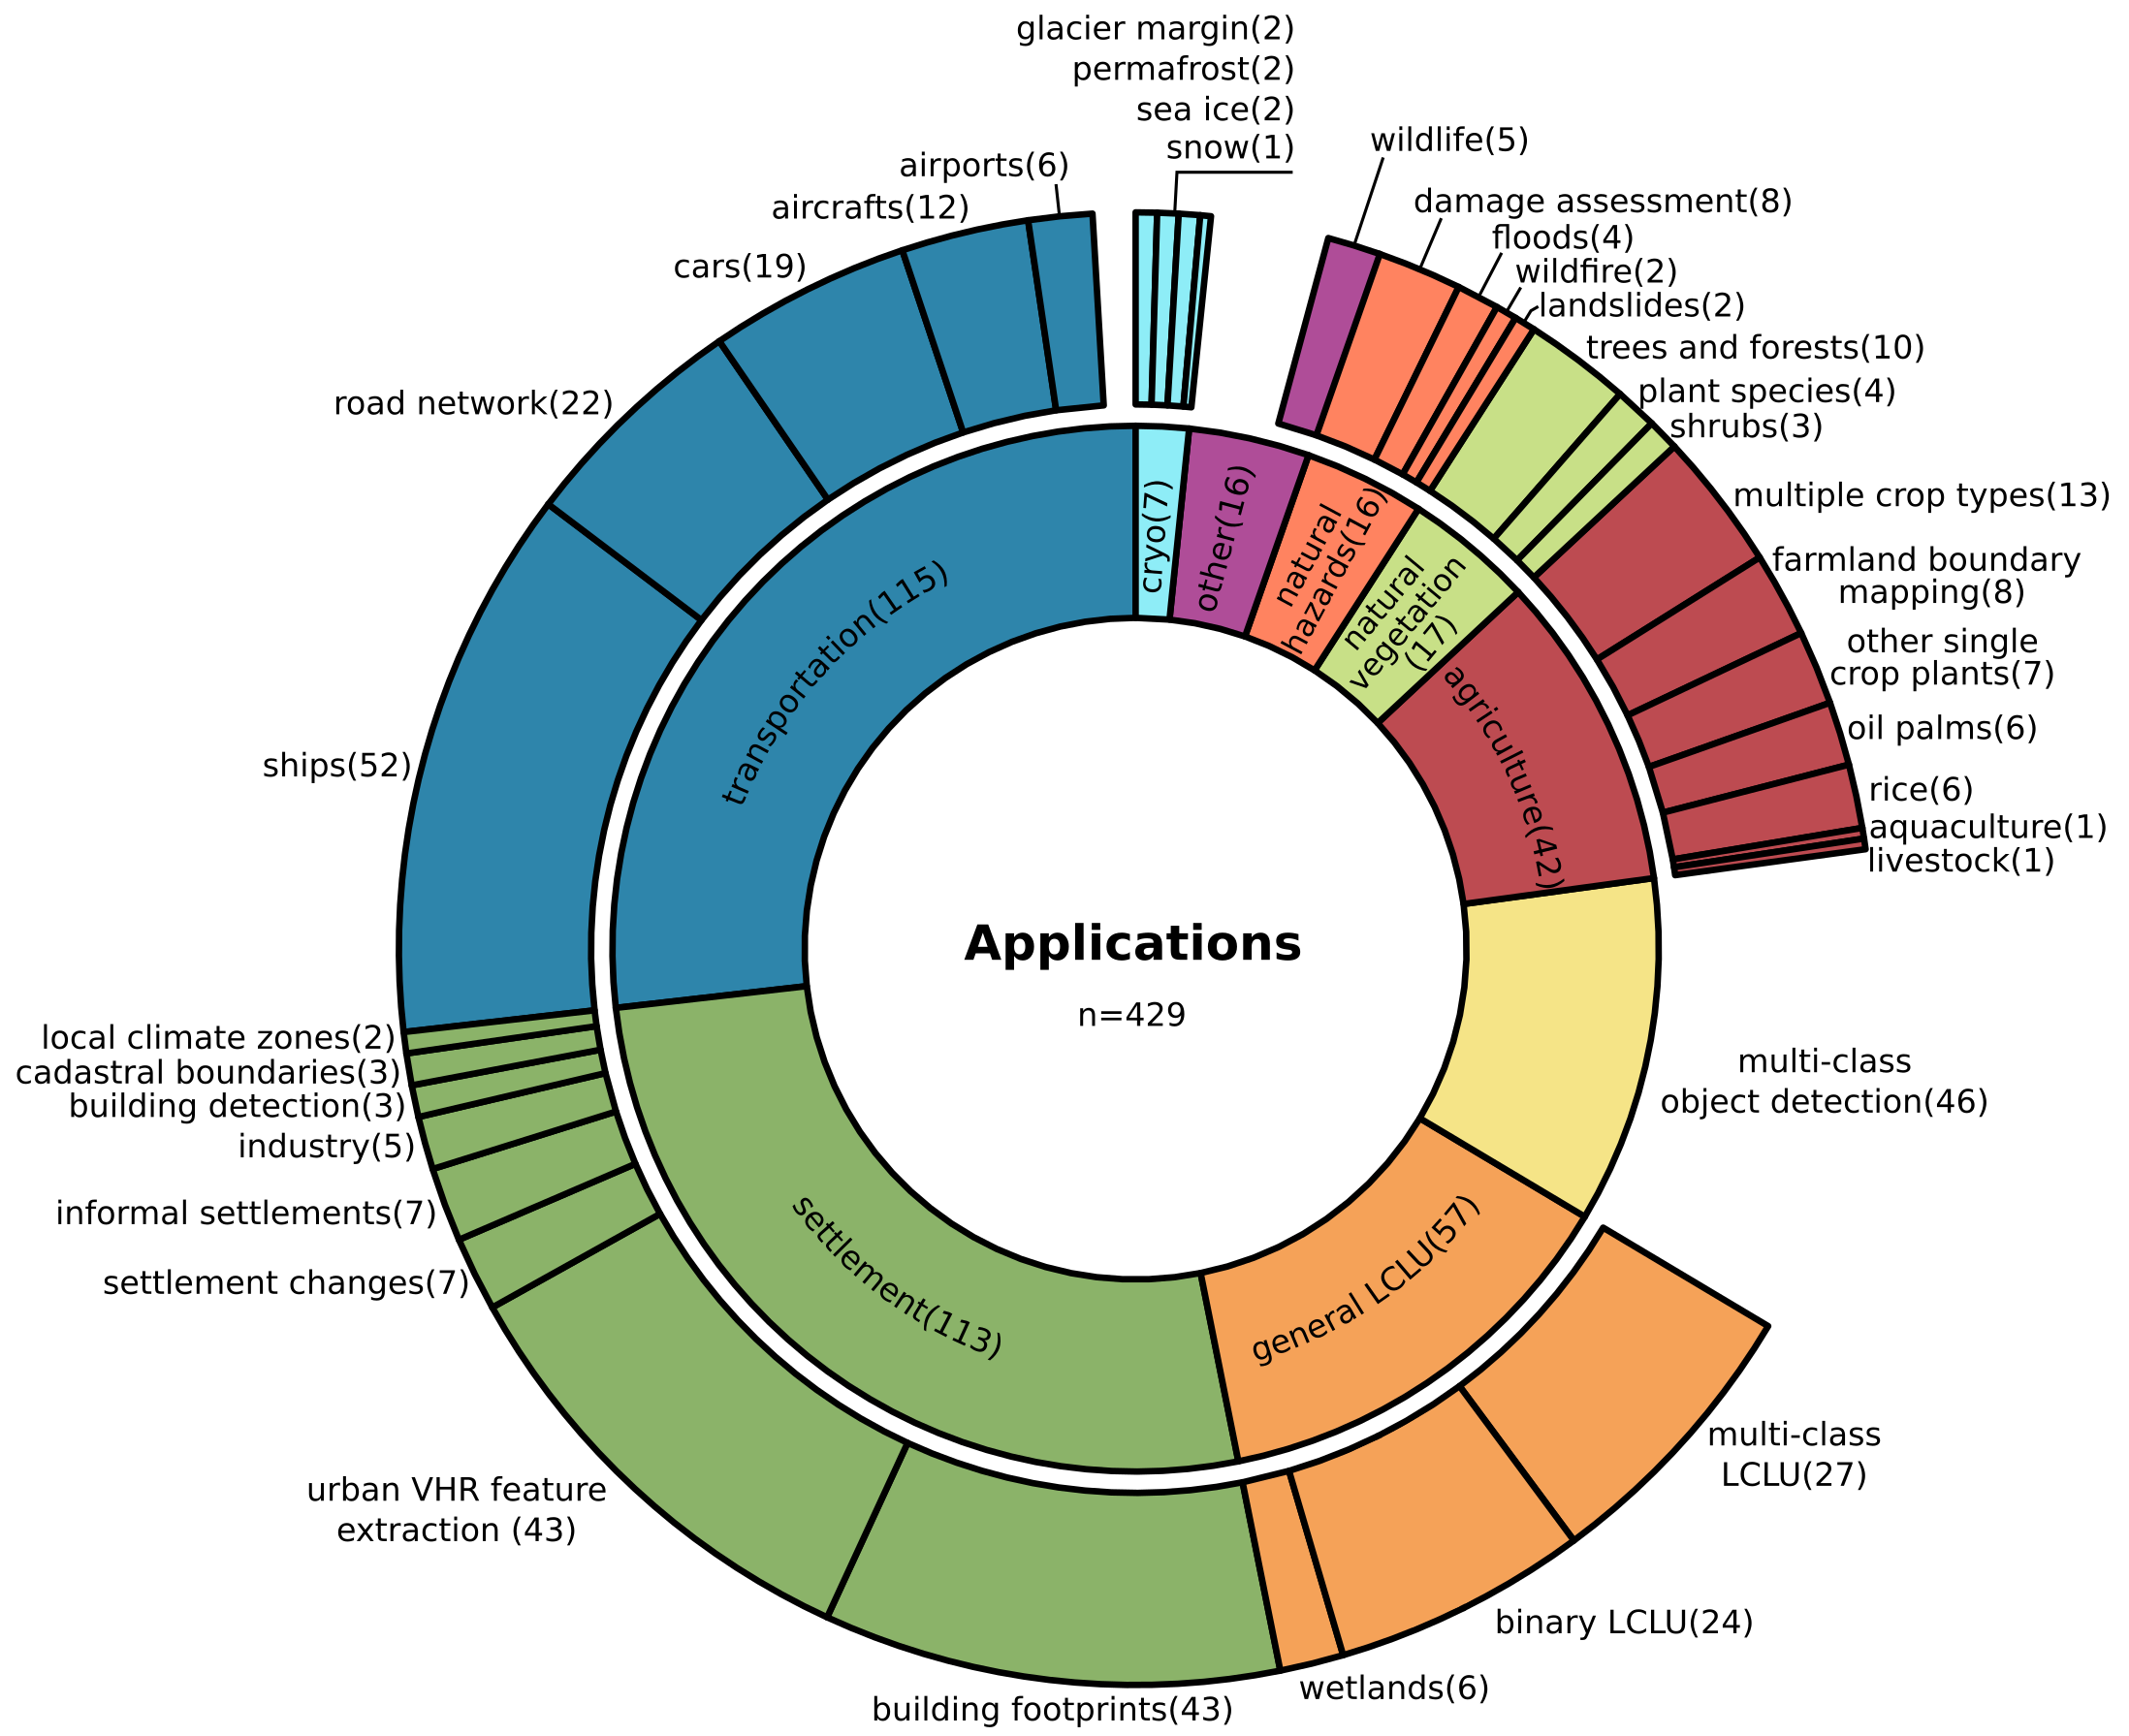
\includegraphics[width=1\textwidth]{Images/RevisionAreas.png}
    \end{center}
    \caption{Aplicaciones destacadas de la inteligencia artificial en la segmentación semántica y la detección de objetos dentro del ámbito de la teledetección.}
    \reference{Datos tomados de \citeA{hoeser2020object}.}
    \label{fig:RevisionAreas}
\end{figure}

Sin embargo, pese a los avances en la aplicación de la inteligencia artificial en la teledetección, como se evidencia en la Figura~\ref{fig:RevisionAreas}, aún se observa una representación mínima de investigaciones enfocadas en la criósfera y los ecosistemas de montaña. Este déficit puede atribuirse, en parte, a la estandarización de técnicas basadas en el cálculo de índices espectrales. Los glaciares, al poseer una firma espectral distintiva, son relativamente sencillos de detectar en comparación con otros elementos \cite{dietz2012remote}. No obstante, la complejidad emerge al mapear glaciares cubiertos de escombros o glaciares rocosos debido a sus diferencias espectrales con respecto a otros tipos de glaciares y su similitud espectral con el terreno circundante \cite{nijhawan2018hybrid}. En la actualidad, estos desafíos suelen abordarse mediante procesos manuales, tal y como se describe en la Sección~\ref{sec:SituacionProblematica}, resultando en procedimientos extensos, laboriosos y costosos.

En este contexto, la presente investigación buscará contribuir a este campo de estudio poco explorado, mediante el desarrollo de un modelo semiautomático de segmentación semántica de glaciares basado en aprendizaje profundo. Complementariamente, se efectuará una revisión sistemática de los estudios de vanguardia que incorporan inteligencia artificial en el mapeo de glaciares, con la finalidad de brindar a la comunidad científica una perspectiva actualizada de las innovaciones y tendencias emergentes en la aplicación de estas técnicas en la teledetección centrada en los ecosistemas de montaña. Se espera que estos aportes puedan impulsar nuevas investigaciones y aplicaciones basadas en inteligencia artificial en este campo, potenciando la capacidad para monitorizar y entender los cambios y dinámicas en los ecosistemas de montaña.

\subsection{Justificación práctica}

En América Latina, países como Perú, Chile, Argentina y Colombia disponen de instituciones especializadas en el estudio y seguimiento de glaciares y ecosistemas de montaña \cite{inaigem2017manual, DGA2022, castro2014manual, ospina2022metodologia}. Estas entidades cuentan con equipos multidisciplinarios responsables de la creación de sus respectivos inventarios de glaciares.

Los inventarios de glaciares son instrumentos cruciales para las administraciones gubernamentales a nivel mundial, facilitando la implementación de políticas de respuesta al rápido declive de la superficie glaciar en regiones específicas \cite{barella2022combined}. La actualización constante de estos inventarios es esencial, puesto que la calidad y la contemporaneidad de los datos tienen una incidencia directa en la eficacia de las estrategias para la conservación de los glaciares \cite{alifu2020machine, lu2021novel, xie2022progressive}.

Sin embargo, la actualización de un inventario de glaciares es un proceso largo y costoso debido a su inherente complejidad \cite{yan2021glacier}. Este proceso comprende varias etapas, incluyendo la recopilación de información histórica y geoespacial, el análisis de gabinete, la validación en campo, y finalmente, la publicación de los resultados \cite{barcaza2017glacier}. Es por tal motivo que países como Perú han establecido un intervalo de actualización de cinco años para su inventario de glaciares \cite{inaigem2018inventario}, lo que supone una desventaja considerando que, el 86\% de los glaciares en Perú posee una superficie menor a 1 $km^2$, siendo los más susceptibles a los efectos del cambio climático. \cite{reserva2021}.

En ese contexto, la presente investigación busca aportar en la optimización del uso de recursos mediante el incremento de la efectividad en el mapeo semiautomático de glaciares limpios y cubiertos mediante el desarrollo un modelo de segmentación semántica basado en aprendizaje profundo.

Se busca, además, establecer un punto de referencia para la adaptación de nuevas técnicas basadas en el uso de inteligencia artificial en las metodologías empleadas para la elaboración de inventarios de glaciares en los países de la región.